\documentclass[twoside,11pt]{report}

% Any additional packages needed should be included after jmlr2e.
% Note that jmlr2e.sty includes epsfig, amssymb, natbib and graphicx,
% and defines many common macros, such as 'proof' and 'example'.
%
% It also sets the bibliographystyle to plainnat; for more information on
% natbib citation styles, see the natbib documentation, a copy of which
% is archived at http://www.jmlr.org/format/natbib.pdf

\usepackage{jmlr2e}
% \usepackage[utf8]{inputenc}%
% \usepackage{tikz}
% \usepackage{cfr-lm}%
\usepackage[T1]{fontenc}%
\usepackage{physics}
\usepackage{amsmath}
% \usepackage{amssymb}
% \usepackage{graphicx}
% \usepackage[margin=3cm]{geometry}
% \usepackage{changepage}
\usepackage{fontspec}
\usepackage{minted}
\usepackage{tcolorbox}
\usepackage{lmodern}
\usepackage{xcolor}
\usepackage{lettrine}
% \usepackage{fontawesome}
\usemintedstyle{perldoc}
\usepackage{hyperref}
\hypersetup{colorlinks=false, pdfborder={0 0 0},  }
\usepackage{fancyhdr}
\usepackage{wrapfig}
\usepackage{adjustbox}



\newtcbox{\codebox}[1][black]{on line, arc=2pt,colback=#1!10!white,colframe=white, before upper={\rule[-3pt]{0pt}{10pt}},boxrule=1pt, boxsep=0pt,left=2pt,right=2pt,top=1pt,bottom=.5pt}
\newtcbox{\deloppg}[1][black]{on line, arc=2pt,colback=#1!10!white,colframe=white, before upper={\rule[-2pt]{0pt}{0pt}},boxrule=0pt, boxsep=0pt,left=.49\linewidth,right=.49\linewidth,top=4pt,bottom=3pt}


\newcommand\blfootnote[1]{ \begingroup \renewcommand\thefootnote{}\footnote{#1} \addtocounter{footnote}{-1} \endgroup }
% \definecolor{antwhite}{HTML}{323333}
\newcommand{\code}[3][]{\codebox{\mintinline[#1]{#2}{#3}}}



% \setmainfont{FreeSans}
% \setmainfont{SF Pro Display}
% \setmainfont{IBM Plex Sans}
% \setmainfont{TeX Gyre Heros}
% \setmainfont{Inter}
% \setmainfont{Iosevka Quasi}

% \setmonofont{Iosevka Custom Extended}
% \setmonofont{JetBrainsMono Nerd Font}
\setmonofont[Scale=MatchLowercase]{SF Mono}






% Definitions of handy macros can go here

\newcommand{\dataset}{{\cal D}}
\newcommand{\fracpartial}[2]{\frac{\partial #1}{\partial  #2}}

% Heading arguments are {volume}{year}{pages}{submitted}{published}{author-full-names}

% \jmlrheading{1}{2000}{1-48}{4/00}{10/00}{https://github.com/bragewiseth/MachineLearningProjects}

% Short headings should be running head and authors last names

\ShortHeadings{\url{https://github.com/bragewiseth/MachineLearningProjects}}{\url{https://github.com/bragewiseth/MachineLearningProjects}}
\firstpageno{1}



\title{{\huge Project 1}}
\author{\name Eirik J. \email eirk@ifi.uio.no \\
       \name Felix H.  \email felixch@ifi.uio.no \\
       \name Brage W. \email bragewi@ifi.uio.no}
\date{\today}											% Date
\makeatletter






% \date{\today}

\begin{document}

%%%%%%%%%%%%%%%%%%%%%%%%%%%%%%%%%%%%%%%%%%%%%%%%%%%%%%%%%%%%%%%%%%%%%%%%%%%%%%%%%%%%%%%%%

\begin{titlepage}
	\centering
    \vspace*{0.5 cm}
    
\includegraphics[scale = 0.75]{uio.jpg}\\[1.0 cm]	% University Logo
    \textsc{\LARGE University of Oslo}\\[2.0 cm]	    % University Name
	\textsc{\Large FYS-STK3155}\\[0.5 cm]				% Course Code
	\rule{\linewidth}{0.2 mm} \\[0.4 cm]
	{ \huge \bfseries \@title}\\
	\rule{\linewidth}{0.2 mm} \\[1.5 cm]

	\begin{minipage}{0.4\textwidth}
		\begin{flushleft} \normalsize
			Eirik\\
            Felix\\
            Brage Wiseth\\
			\end{flushleft}
			\end{minipage}~
			\begin{minipage}{0.4\textwidth}
			\begin{flushright} \normalsize
        \textsc{
		  eirik@ifi.uio.no\\
          felix@ifi.uio.no\\
          bragewi@ifi.uio.no\\
        }
		\end{flushright}
        
	\end{minipage}\\[2 cm]
	\@date\\
    \vspace*{25mm}
    \urlstyle{rm}
    \textsc{\url{https://github.com/bragewiseth/MachineLearningProjects}}
	
	
    
    
    
    
	
\end{titlepage}
\nocite{*}
% \maketitle
\newpage
\tableofcontents
\newpage




\begin{abstract}%   <- trailing '%' for backward compatibility of .sty file
\lettrine{I}{}n this paper, we delve into the realm of machine learning model optimization and evaluation. 
Our study encompasses various regression techniques, including Ordinary Least Squares (OLS), Ridge, and 
Lasso regression, to analyze their effectiveness in handling simple and more complex datasets. Additionally, 
we employ bootstrap resampling and cross-validation methodologies to rigorously assess model performance 
and enhance generalization.
A significant portion of our investigation is dedicated to understanding the delicate balance between 
bias and variance. We explore how regularization methods like Ridge and Lasso impact bias-variance trade-offs, 
offering insights into the stability and predictive power of these models. Furthermore, we provide empirical 
evidence of the benefits of cross-validation and bootstrap techniques in mitigating overfitting and improving 
model robustness. We found that \{ ..results.. \}. Additionally we verify and compare our findings with well 
established theory and libraris such as SKLearn.
\end{abstract}
\begin{keywords}
    Linear Regression, Scaling, Bias \& Variance 
\end{keywords}









\section{Introduction}

Machine learning has emerged as a powerful tool in data analysis, providing the ability to uncover complex 
patterns and relationships in diverse datasets. But, at its core, machine learning is all about finding 
functions that capture the underlying structure of the data. The use of machine learning algorithms 
to approximate functions is the essence of this paper.\\

Our motivation for this research lies in the exploration of machine learning techniques to approximate 
the terrain on our planet, which can perhaps be described by such a function. Earth's terrain exhibits 
peaks and troughs, hills and valleys, much like some polynomial functions. Fortunately, we can employ 
standard linear regression techniques to approximate polynomials, but the terrain presents its own set 
of challenges. Firstly, the terrain's true underlying function may not be a polynomial at all, and its complexity may 
vary significantly from one location to another. Secondly, our landscape is teeming with small, intricate 
details. Some regions are characterized by flat and smooth surfaces, while others are marked by rough and 
uneven terrain. Focusing too much on these minute details can lead to model overfitting, making it crucial 
to strike a careful balance between model complexity and generalization.
In this context, regularization and resampling techniques, including Ridge and Lasso regression with bootstrap
and cross validation, have proven indispensable. By introducing regularization and resampling, we aim to find 
the sweet spot between bias and Variance. And getting the best predictions we can with our assumptions.\\
To embark on this exploration, we will begin with a simpler case: "Franke's function." which mimics our real terrain
data. This function 
serves as a foundational starting point, allowing us to assess our model's performance in a controlled 
environment before venturing into the complexity of real-world terrain data. Through this gradual progression, 
we provide ourselves wih a framework that can be applied to more complex and varied real-world terrain datasets.\\

\textbf{Data}: We begin by introducing the dataset used for our analysis, highlighting data collection and preprocessing procedures. 
Understanding the characteristics of the terrain data is fundamental to our modeling endeavor.\\
\textbf{Methods and Scaling}: Next, we delve into the methodology, encompassing the implementation of polynomial regression 
models and the application of regularization techniques such as Ridge and Lasso. Additionally, we will discuss the 
importance of proper scaling for model stability and convergence.\\
\textbf{Bias-Variance Trade-off}: A significant portion of our study will revolve around the critical concept of bias and 
variance. We'll explore how regularization methods influence this trade-off and delve into the fine balance between 
model complexity and generalization.\\
\textbf{Results}: In this section, we will present the outcomes of our experiments, showcasing the performance of different 
models and regularization techniques. Through empirical evidence, we aim to provide insights into the effectiveness of our approach.\\
\textbf{Conclusion}: Finally, we will summarize the key findings and their implications for terrain modeling with machine learning. 
Our conclusion will underscore the importance of regularization in achieving accurate representations of complex terrains and 
provide a perspective on future research directions.

\begin{center}
    \scriptsize code for generating all figures and data can be found at 
\href{https://github.com/bragewiseth/MachineLearningProjects/tree/main/project1/src}{\tt \textsc{/MachineLearningProjects/project1/src} }
\end{center}








\section{Data}
\label{sec:data}

\begin{wrapfigure}{r}{0.3\textwidth}
\begin{center}
    \begin{adjustbox}{clip,trim=4cm 3.4cm 3cm 4.8cm, max width=0.3\textwidth}
    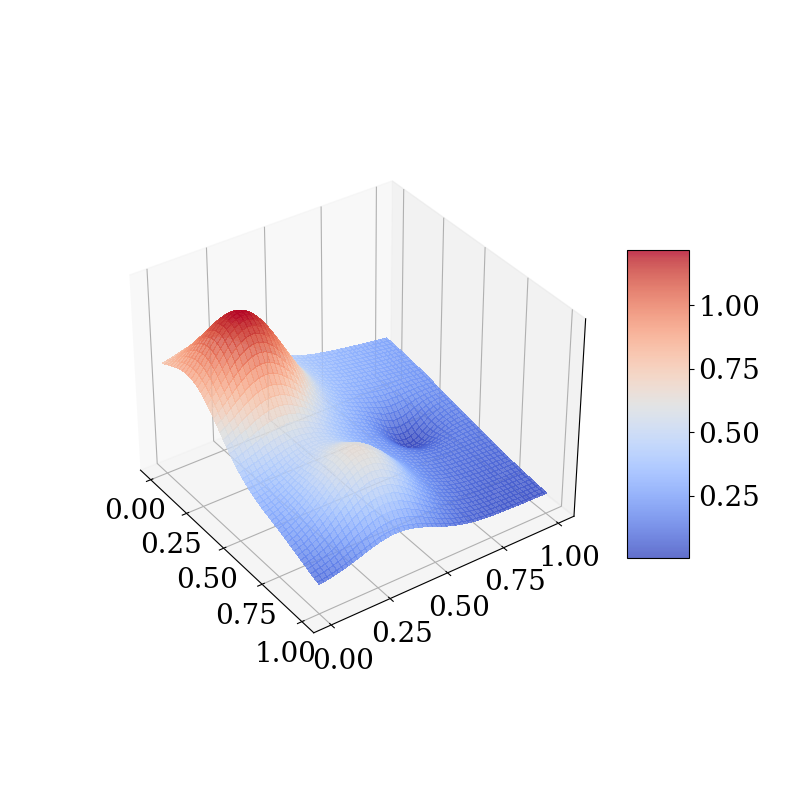
\includegraphics{../runsAndAdditions/trueFunction.png}
    \end{adjustbox}
    \caption{\small franke's function with noise}
    \end{center}
\end{wrapfigure}

\begin{wrapfigure}{l}{0.3\textwidth}
    \caption{\small franke's function}
    \begin{center}
    \begin{adjustbox}{clip,trim=4cm 3.4cm 3cm 4.8cm, max width=0.3\textwidth}
        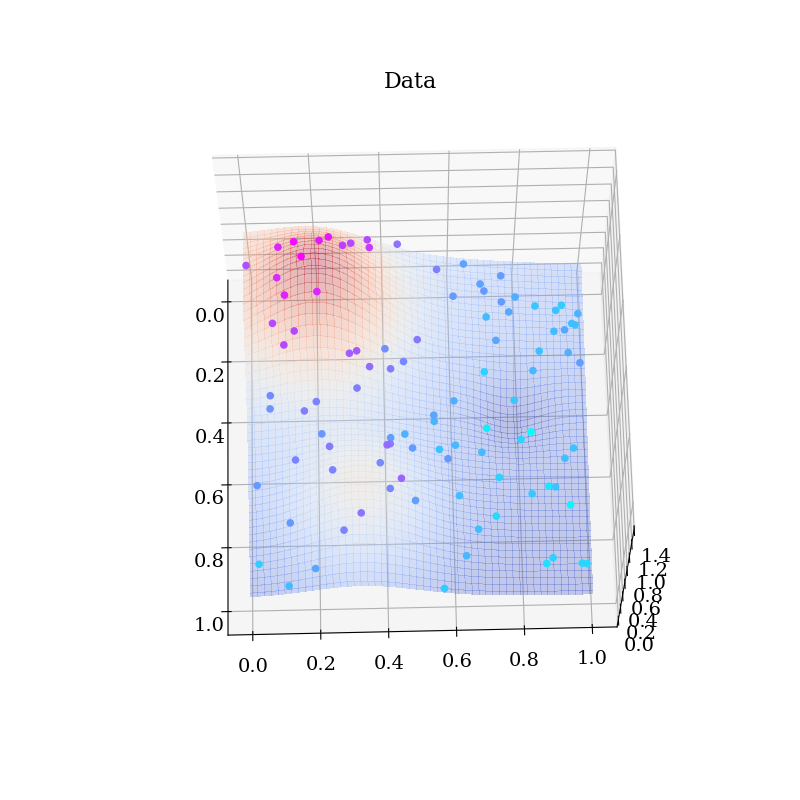
\includegraphics{../runsAndAdditions/synthDataTop.png}
    \end{adjustbox}
    \end{center}
\end{wrapfigure}

\begin{figure}
    \begin{center}
        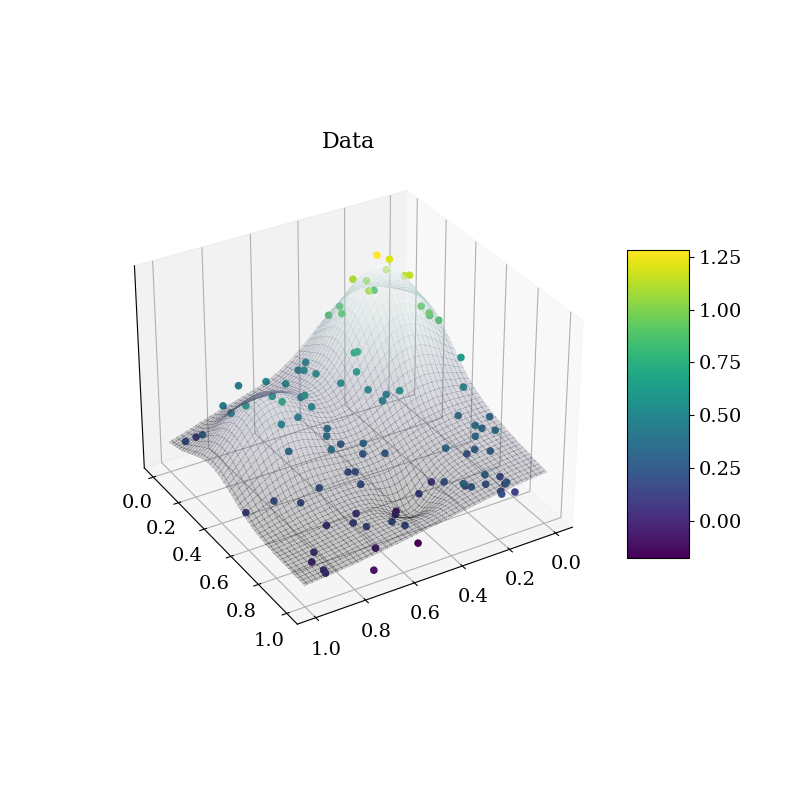
\includegraphics[width=0.95\textwidth]{../runsAndAdditions/synthDataSide.png}
    \end{center}
\end{figure}










\section{linear regression models }
\label{sec:models}



$$
mse(\mathbf{y},\mathbf{\tilde{y}}) = \frac{1}{n}
\sum_{i=0}^{n-1}(y_i-\tilde{y}_i)^2,
$$
$$
r^2(\mathbf{y}, \tilde{\mathbf{y}}) = 1 - \frac{\sum_{i=0}^{n - 1} (y_i - \tilde{y}_i)^2}{\sum_{i=0}^{n - 1} (y_i - \bar{y})^2},
$$

$$
\bar{y} =  \frac{1}{n} \sum_{i=0}^{n - 1} y_i.
$$








\subsection{Ordinary Least Squares (OLS)}
\label{sec:ols}







\subsection{Ridge Regression}
\label{sec:ridge}







\subsection{lasso Regression}
\label{sec:lasso}


\begin{figure}[!h]
    \begin{center}
    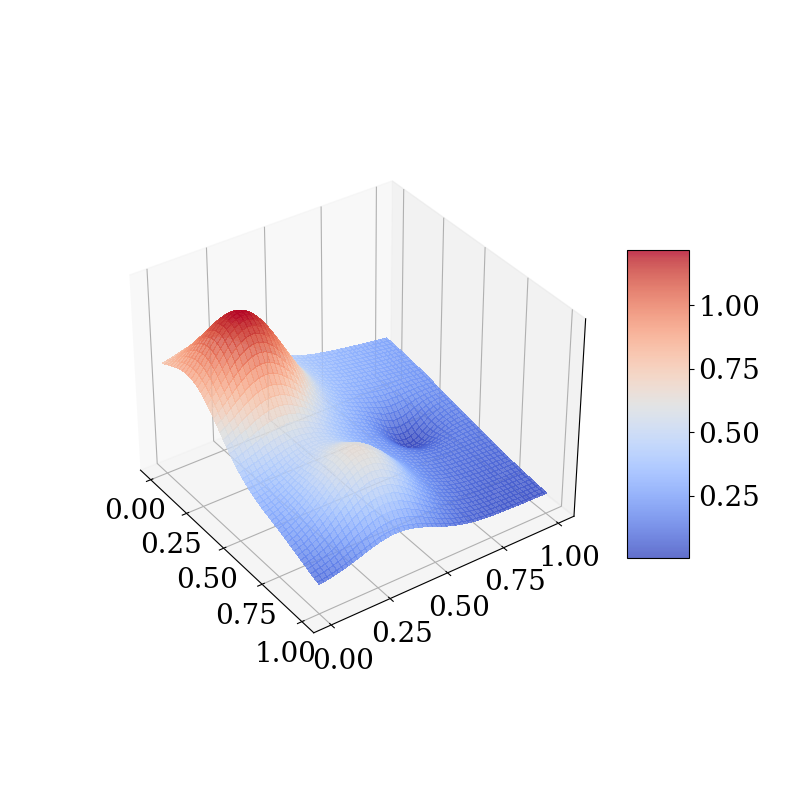
\includegraphics{../runsAndAdditions/trueFunction.png}
    \end{center}
\end{figure}
\begin{figure}[!h]
    \begin{center}
        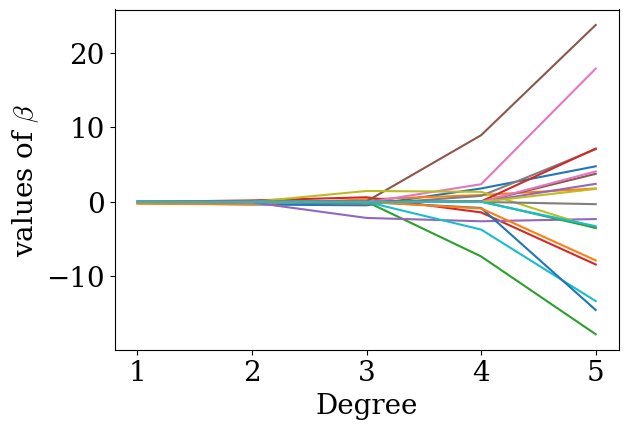
\includegraphics{../runsAndAdditions/betaOverOrderOLS.png}
    \end{center}
\end{figure}










\subsection{Scaling}
\label{sec:scaling}


\begin{table}[!h]
\caption{unscaled sample design matrix fitting one-dimensional polynomial of degree 5}
\tt
\centering
% \resizebox{0.6\textwidth}{!}{%
\begin{tabular}{llllll}
    1. &     0.  &    0.  &    0.   &   0.   &   0.     \\
    1. &     0.25 &   0.0625 & 0.01562& 0.00391& 0.00098\\
    1.    &  0.5     &0.25 &   0.125 &  0.0625 & 0.03125\\
    1.   &   0.75  &  0.5625 & 0.42188 &0.31641& 0.2373 \\
    1.  &    1.   &   1.  &    1.  &    1.    &  1.
\end{tabular}%
% }
\end{table}
\begin{table}[!h]
\caption{scaled sample design matrix fitting one-dimensional polynomial of degree 5}
\tt
\centering
% \resizebox{0.6\textwidth}{!}{%
\begin{tabular}{llllll}
     0. &     -1.41421& -1.0171&  -0.83189& -0.728 &  -0.66226\\
     0.  &    -0.70711& -0.84758& -0.7903 & -0.71772& -0.65971\\
     0.  &     0.    &  -0.33903& -0.49913& -0.56348& -0.58075\\
     0.  &     0.70711&  0.50855&  0.29116 & 0.10488& -0.0433 \\
     0.  &     1.41421&  1.69516 & 1.83016 & 1.90431&  1.94603
\end{tabular}%
% }\\
\end{table}
\begin{table}[h]
\centering
\resizebox{0.7\textwidth}{!}{%
\begin{tabular}{ll}
mse for ols on unscaled data:    &   \texttt{0.010349396022903145} \\
mse for ols on scaled data:      &   \texttt{0.010349396024145656} \\
mse for ridge on unscaled data:  &   \texttt{0.02106077418650843} \\
mse for ridge on scaled data:    &   \texttt{0.01782525371566323}
\end{tabular}%
}
\end{table}
At first glance, there isn't a big difference between the unscaled data (xunscaled) and the scaled data (xscaled). 
This is because the original data was already close to having a mean close to zero and not being spread out too much. 
So, you might think that scaling the data isn't necessary.
However, when we introduce polynomial terms, we notice that some values in xunscaled become extremely small, for example, 
0.15 turns into 0.00001. This means that the columns of xunscaled have vastly different orders of magnitude, and this calls 
for scaling to bring them back to a similar scale.
If we don't scale, the coefficients (β) can range widely, from -50 to 48. But when we scale the data, this range narrows 
down to -10 to 13. Now, this alone might not seem like a strong reason to scale the data, especially when we use plain 
linear regression (OLS), as it doesn't change the Mean Squared Error (MSE) much.

However, things change when we use Ridge regression. In Ridge, the regularization cost depends on the magnitude of βi.
With unscaled data, where βi varies a lot, some coefficients get penalized more than others. This results in a 
significantly higher MSE for unscaled data compared to scaled data in Ridge regression.
So, to make it easier to tune the regularization parameter (λ) and to ensure fair treatment of coefficients in Ridge regression, 
it's a good idea to scale the data. This not only simplifies the regularization process but also leads to better predictive performance.










\section{Results and Discussion}
\label{sec:resultsdiscussion}


\textbf{Note to self} på real data tester vi ikke alle hyperparametere, det tar alt for lang tid
vi bruker den beste k fra synthetic data of gjør binærsøk på lambda og degrees 


we see that ols remains constant since it is not a function of λ. for the mse from the training set we se that 
the mse wil increase for larger values of λ for rigde regression. this is expected since the ols wil give the 
best approximation for the data it has been trained on (compared to rigde), while rigde punishes the weights 
from becomming too large and therefore gives a not so tight fit. this can explain why rigde does better than 
ols for some values of λ. as stated before the ols wil try to fit the model to the best of its ability to the 
training data, this includes the noise which might not generalize to the test set, hence giving rigde a greater score. 
the term for this is called ***overfitting***. and balancing between overfitting and underfitting is called the ***bias variance tradeoff***. 










\subsection{confidence interval}
\label{sec:confidenceinterval}

the assumption we have made is that there exists a continuous function f (x)
and a normal distributed error ε ∼ n (0, σ2) which describes our data
y = f (x) + ε
we then approximate this function f (x) with our model ˜y from the solution
of the linear regression equations (ordinary least squares ols), that is our
function f is approximated by ˜y where we minimized (y − ˜y)2, with
˜y = xβ.
the matrix x is the so-called design or feature matrix.
yi ∼ n (xi,∗ β, σ2), that is y follows a normal distribution with mean
value xβ and variance σ2.
we can use this when we define a so-called confidence interval
for the parameters β. a given parameter βj is given by the diagonal matrix
element of the above matrix.
\ref{app:confidenceinterval}







\section{bias \& variance}
\label{sec:biasvariance}


\begin{align*}
    \text{var}(\mathbf{\tilde{y}}) &= \mathbb{e}\left[\left(\tilde{\mathbf{y}}-\mathbb{e}\left[\mathbf{\tilde{y}}\right]\right)^2\right] = \mathbb{e}[\mathbf{\tilde{y}}^2] - \mathbb{e}[\mathbf{\tilde{y}}]^2\\
    \mathbb{e}[\mathbf{\tilde{y}}^2] &= \mathbb{e}[\mathbf{\tilde{y}}]^2 + \text{var}(\mathbf{\tilde{y}})
\end{align*}


\begin{align*}
\mathbb{e}[\mathbf{y}^2] & = \mathbb{e}[\mathbf{f} + \mathbf{\epsilon}]^2 = \mathbb{e}[\mathbf{f}^2 + 2\mathbf{f}\mathbf{\epsilon} + \mathbf{\epsilon}^2]\\
& = \mathbb{e}[\mathbf{f}^2] + 2\mathbb{e}[\mathbf{f}\mathbf{\epsilon}] + \mathbb{e}[\mathbf{\epsilon}^2]\\
& = \mathbb{e}[\mathbf{f}^2] + 2\mathbb{e}[\mathbf{f}]\mathbb{e}[\mathbf{\epsilon}] + \mathbb{e}[\mathbf{\epsilon}^2]\\
& = \mathbb{e}[\mathbf{f}^2]  + \sigma^2
\end{align*}


\begin{align*}
\mathbb{e}[\mathbf{y\tilde{y}}] & = \mathbb{e}[\mathbf{f\tilde{y}} + \mathbf{\epsilon\tilde{y}}]\\
& = \mathbb{e}[\mathbf{f\tilde{y}}] + \mathbb{e}[\mathbf{\epsilon\tilde{y}}]\\
& = \mathbb{e}[\mathbf{f\tilde{y}}] + \mathbb{e}[\mathbf{\epsilon}]\mathbb{e}[\mathbf{\tilde{y}}]\\
& = \mathbf{f}\mathbb{e}[\mathbf{\tilde{y}}]
\end{align*}


\begin{align*}
\mathbb{e}\left[(\mathbf{y}-\mathbf{\tilde{y}})^2\right] & = \mathbb{e}[\mathbf{y}^2] - 2\mathbb{e}[\mathbf{y\tilde{y}}] + \mathbb{e}[\mathbf{\tilde{y}}^2]\\
& = \mathbf{f}^2 + \sigma^2 - 2\mathbf{f}\mathbb{e}[\mathbf{\tilde{y}}] + \mathbb{e}[\mathbf{\tilde{y}}^2]\\
& = \mathbf{f}^2 + \sigma^2 - 2\mathbf{f}\mathbb{e}[\mathbf{\tilde{y}}] + \mathbb{e}[\mathbf{\tilde{y}}]^2 + \text{var}(\mathbf{\tilde{y}})\\
& = (\mathbf{f} - \mathbb{e}[\mathbf{\tilde{y}}])^2 + \text{var}(\mathbf{\tilde{y}}) + \sigma^2\\
\end{align*}


\begin{align*}
\mathrm{bias}[\tilde{y}]& =\mathbb{e}\left[\left(\mathbf{y}-\mathbb{e}\left[\mathbf{\tilde{y}}\right]\right)^2\right] = \mathbb{e}[\mathbf{y}^2] - 2\mathbb{e}[\mathbf{y}]\mathbb{e}[\mathbf{\tilde{y}}] + \mathbb{e}[\mathbf{\tilde{y}}^2]\\
& = \mathbf{f}^2 + \sigma^2 - 2\mathbf{f}\mathbb{e}[\mathbf{\tilde{y}}] + \mathbb{e}[\mathbf{\tilde{y}}]^2\\
& = (\mathbf{f} - \mathbb{e}[\mathbf{\tilde{y}}])^2 + \sigma^2\\
\end{align*}


to find $\mathbb{e}[\mathbf{\tilde{y}}]$ we can use bootstrap to get different samples for $\mathbf{\tilde{y}}$ and then take the mean of that distribution.
the term \emph{variance} refers to how spread out our observations are. we can for our case think of the observations $\tilde{y}_i$
as either individual predictions, or the mean of predictions from one test set.\\
in a sense the bias resembles the mathematical defninition for variance, we can see that the bias term is a distance measure of $\mathbf{y}$ from the expected value of $\mathbf{\tilde{y}}$. if we take the individual observations approach this can be tough of as a high bias will then result in a large band around $\mathbf{\tilde{y}}$ in which $y_i$ will exist. the variance term is a measure of how much the $\mathbf{\tilde{y}}$ varies around its own mean. in other terms a high variance model will experience large variance in the predicted values $\mathbf{\tilde{y}}$ from one test set to another. or as a result of this a large variance in score if you will. now these two terms are in a sense opposites, it is likely that a model with high bias will have low variance and vice versa. this is something we as designers of the model get to tune, if we value a lower bias more than we value a low variance or vice versa, we can choose a model accordingly






































% \acks{}



% APPENDIX

%
%
\newpage
\appendix
\phantomsection%
\addcontentsline{toc}{section}{Appendix}
\section*{Appendix}
\label{app:appendix}

appendix



\phantomsection%
\addcontentsline{toc}{subsection}{Analytical Least Squares}
\subsection*{Derivation of The Optimal Parameters $\beta$}
\label{app:OptimalBeta}

OLS

The expression for the standard Mean Squared Error (MSE) which we used to define our cost function and the equations for the ordinary least squares (OLS) method, was given by the
optimization problem


$$
{\displaystyle \min_{\mathbf{\beta}\in {\mathbb{R}}^{p}}}\frac{1}{n}\left\{\left(\mathbf{y}-\mathbf{X}\mathbf{\beta}\right)^T\left(\mathbf{y}-\mathbf{X}\mathbf{\beta}\right)\right\}.
$$

can also be written as 

$$
{\displaystyle \min_{\mathbf{\beta}\in
{\mathbb{R}}^{p}}}\frac{1}{n}\sum_{i=0}^{n-1}\left(y_i-\tilde{y}_i\right)^2=\frac{1}{n}\vert\vert \mathbf{y}-\mathbf{X}\mathbf{\beta}\vert\vert_2^2,
$$


$$
{\displaystyle \min_{\mathbf{\beta}\in
{\mathbb{R}}^{p}}}\frac{1}{n}\vert\vert \mathbf{y}-\mathbf{X}\mathbf{\beta}\vert\vert_2^2
$$


$$
\hat{\mathbf{\beta}}_{\mathrm{OLS}} = \left(\mathbf{X}^T\mathbf{X}\right)^{-1}\mathbf{X}^T\mathbf{y},
$$



Ridge



We know that 
$$
{\displaystyle \min_{\mathbf{\beta}\in
{\mathbb{R}}^{p}}}\frac{1}{n} \vert\vert\mathbf{y}- \mathbf{X}\mathbf{\beta}\vert\vert_2^2 = \frac{2}{n} \mathbf{X}^T\mathbf{X}\mathbf{\beta}-\frac{2}{n}\mathbf{X}^T\mathbf{y}
$$

The minimization of ridge addition alone is
$${\displaystyle \min_{\mathbf{\beta}\in
{\mathbb{R}}^{p}}}\frac{1}{n} \lambda \vert\vert \mathbf{\beta}\vert\vert_2^2 = \frac{2}{n} \lambda \mathbf{\beta}
$$

adding these two we get
$$
    \frac{\partial \left[\frac{1}{n}\vert\vert \mathbf{y}-\mathbf{X}\mathbf{\beta}\vert\vert_2^2+\lambda\vert\vert \mathbf{\beta}\vert\vert_2^2\right]}
    {\partial{\mathbf{\beta}}} = 0 
    = \frac{2}{n}\left(\mathbf{X}^T\mathbf{X}+\lambda\mathbf{I}\right)
    \mathbf{\beta}-\frac{2}{n}\mathbf{X}^T\mathbf{y} \implies \beta = \left(\mathbf{X}^T\mathbf{X}+\lambda\mathbf{I}\right)^{-1}\mathbf{X}^T\mathbf{y}
$$


$$
{\displaystyle \min_{\mathbf{\beta}\in
{\mathbb{R}}^{p}}}\frac{1}{n}\vert\vert \mathbf{y}-\mathbf{X}\mathbf{\beta}\vert\vert_2^2+\lambda\vert\vert \mathbf{\beta}\vert\vert_2^2
$$



$$
{\displaystyle \min_{\mathbf{\beta}\in
{\mathbb{R}}^{p}}}\frac{1}{n}\sum_{i=0}^{n-1}\left(y_i-\tilde{y}_i\right)^2=\frac{1}{n}\vert\vert \mathbf{y}-\mathbf{X}\mathbf{\beta}\vert\vert_2^2,
$$




$$
{\displaystyle \min_{\mathbf{\beta}\in
{\mathbb{R}}^{p}}}\frac{1}{n}\vert\vert \mathbf{y}-\mathbf{X}\mathbf{\beta}\vert\vert_2^2+\lambda\vert\vert \mathbf{\beta}\vert\vert_2^2
$$









$$
\hat{\mathbf{\beta}}_{\mathrm{Ridge}} = \left(\mathbf{X}^T\mathbf{X}+\lambda\mathbf{I}\right)^{-1}\mathbf{X}^T\mathbf{y},
$$





\phantomsection%
\addcontentsline{toc}{subsection}{SVD}
\subsection*{SVD}
\label{app:svd}



Use the singular value decomposition of an $n\times p$ matrix $\mathbf{X}$ (our design matrix)

$$
\mathbf{X}=\mathbf{U}\mathbf{\Sigma}\mathbf{V}^T,
$$


where $\mathbf{U}$ and $\mathbf{V}$ are orthogonal matrices of dimensions
$n\times n$ and $p\times p$, respectively, and $\mathbf{\Sigma}$ is an
$n\times p$ matrix which contains the ingular values only. This material was discussed during the lectures of week 35.

Show that you can write the 
OLS solutions in terms of the eigenvectors (the columns) of the orthogonal matrix  $\mathbf{U}$ as


$$
\tilde{\mathbf{y}}_{\mathrm{OLS}}=\mathbf{X}\mathbf{\beta}  = \sum_{j=0}^{p-1}\mathbf{u}_j\mathbf{u}_j^T\mathbf{y}.
$$


$$
\mathbf{X}^T\mathbf{X} = \mathbf{V}\mathbf{\Sigma}^T\mathbf{U}^T\mathbf{U}\mathbf{\Sigma}\mathbf{V}^T = \mathbf{V}\mathbf{\Sigma}^T\mathbf{\Sigma}\mathbf{V}^T = \mathbf{V}\mathbf{\Sigma}^2\mathbf{V}^T
$$

$$
\tilde{\mathbf{y}}_{\mathrm{OLS}} = \mathbf{X}\mathbf{\beta} = \mathbf{X} \left(\mathbf{X}^T \mathbf{X}\right)^{-1} \mathbf{X}^T \mathbf{y}
\\ = \mathbf{U}\mathbf{\Sigma}\mathbf{V}^T \left( \mathbf{V}\mathbf{\Sigma}^2\mathbf{V}^T \right)^{-1} \mathbf{V}\mathbf{\Sigma}^T\mathbf{U}^T \mathbf{y}
\\ = \mathbf{U}\mathbf{\Sigma}\mathbf{V}^T {\mathbf{V}^T}^{-1} {\mathbf{\Sigma}^2}^{-1} \mathbf{V}^{-1}  \mathbf{V}\mathbf{\Sigma}^T\mathbf{U}^T \mathbf{y}
$$

using the orthogonality of $\mathbf{V}$ and $\mathbf{U}$ we get. Multiplying with $\mathbf{\Sigma}$ removes columns from $\mathbf{U}$ with eigenvalues equal to zero.

$$
\tilde{\mathbf{y}}_{\mathrm{OLS}} = \mathbf{U}\mathbf{U}^T \mathbf{y}= \sum_{j=0}^{p-1}\mathbf{u}_j\mathbf{u}_j^T\mathbf{y}
$$




\phantomsection%
\addcontentsline{toc}{subsection}{Confidence Interval}
\subsection*{Math Behind the Confidence Interval section}
\label{app:confidenceInterval}
We can assume that $y$ follows some function $f$ with some noise $\epsilon$

$$
\mathbf{y} = f(\mathbf{x})+\mathbf{\varepsilon}
$$

$$
\mathbf{\tilde{y}} = \mathbf{X}\mathbf{\beta}.
$$

$$
\mathbb{E}(y_i)  =\sum_{j}x_{ij} \beta_j=\mathbf{X}_{i, \ast} \, \mathbf{\beta}
$$

$$
{Var}(y_i)  = \sigma^2
$$

$$
{Var}(\mathbf{\hat{\beta}}) = \sigma^2 \, (\mathbf{X}^{T} \mathbf{X})^{-1}.
$$
$$
\mathbf{y} = f(\mathbf{x}) + \epsilon
$$

$$
\mathbb{E}[\mathbf{y}] = \mathbb{E}[f(\mathbf{x} )+ \epsilon] = \mathbb{E}[f(\mathbf{x})] + \mathbb{E}[\epsilon_i]
$$

The expected value of $\epsilon_i$ is $0$, $f(x)$ is a non-stochastic variable and is approimated by $\mathbf{X}\mathbf{\beta}$

$$
\mathbb{E}[y_i] = \mathbf{X_{i,*}}\mathbf{\beta}
$$

The variance is defined as
\begin{align*}
Var(y_i) &= \mathbb{E}\big[(y_i - \mathbb{E}[y_i])^2\big] = \mathbb{E}\left[y_i^2 - 2y_i\mathbb{E}[y_i] + \mathbb{E}[y_i]^2\right] = \mathbb{E}[y_i^2] - \mathbb{E}[y_i]^2\\
Var(y_i) &= \mathbb{E}\big[\big(\mathbf{X}_{i,*}\mathbf{\beta}\big)^2 + 2\epsilon \mathbf{X}_{i,*}\mathbf{\beta} + \epsilon^2 \big] - (\mathbf{X}_{i,*}\mathbf{\beta})^2\\
Var(y_i) &= (\mathbf{X}_{i,*}\mathbf{\beta})^2 + 2\mathbb{E}[\epsilon]\mathbf{X}_{i,*}\mathbf{\beta} + \mathbb{E}[\epsilon^2] - (\mathbf{X}_{i,*}\mathbf{\beta})^2\\
Var(y_i) &= \mathbb{E}[\epsilon^2] = \sigma^2
\end{align*}
for the expected value of $\mathbf{\beta}$ we can insert the definition of $\mathbf{\beta}$ from earlier


$$
\mathbb{E}[\mathbf{\hat{\beta}}] = \mathbb{E}[ (\mathbf{X}^{\top} \mathbf{X})^{-1}\mathbf{X}^{T} \mathbf{Y}]=(\mathbf{X}^{T} \mathbf{X})^{-1}\mathbf{X}^{T} \mathbb{E}[ \mathbf{Y}]=(\mathbf{X}^{T} \mathbf{X})^{-1} \mathbf{X}^{T}\mathbf{X}\mathbf{\beta}=\mathbf{\beta}
$$


\begin{align*}
Var(\mathbf{\hat{\beta}}) & = \mathbb{E} \{ [\mathbf{\beta} - \mathbb{E}(\mathbf{\beta})] [\mathbf{\beta} - \mathbb{E}(\mathbf{\beta})]^{T} \}
\\
& = \mathbb{E} \{ [(\mathbf{X}^{T} \mathbf{X})^{-1} \, \mathbf{X}^{T} \mathbf{y} - \mathbf{\beta}] \, [(\mathbf{X}^{T} \mathbf{X})^{-1} \, \mathbf{X}^{T} \mathbf{y} - \mathbf{\beta}]^{T} \}
\\
& = (\mathbf{X}^{T} \mathbf{X})^{-1} \, \mathbf{X}^{T} \, \mathbb{E} \{ \mathbf{y} \, \mathbf{y}^{T} \} \, \mathbf{X} \, (\mathbf{X}^{T} \mathbf{X})^{-1} - \mathbf{\beta} \, \mathbf{\beta}^{T}
\\
& = (\mathbf{X}^{T} \mathbf{X})^{-1} \, \mathbf{X}^{T} \, \{ \mathbf{X} \, \mathbf{\beta} \, \mathbf{\beta}^{T} \,  \mathbf{X}^{T} + \sigma^2 \} \, \mathbf{X} \, (\mathbf{X}^{T} \mathbf{X})^{-1} - \mathbf{\beta} \, \mathbf{\beta}^{T}
\\
& = \mathbf{\beta} \, \mathbf{\beta}^{T}  + \sigma^2 \, (\mathbf{X}^{T} \mathbf{X})^{-1} - \mathbf{\beta} \, \mathbf{\beta}^{T}
\, \, \, = \, \, \, \sigma^2 \, (\mathbf{X}^{T} \mathbf{X})^{-1},
\end{align*}



ridge


$$
\mathbb{E} \big[ \hat{\mathbf{\beta}}^{\mathrm{Ridge}} \big]=(\mathbf{X}^{T} \mathbf{X} + \lambda \mathbf{I}_{pp})^{-1} (\mathbf{X}^{\top} \mathbf{X})\mathbf{\beta}.
$$


$$
{Var}[\hat{\mathbf{\beta}}^{\mathrm{Ridge}}]=\sigma^2[  \mathbf{X}^{T} \mathbf{X} + \lambda \mathbf{I} ]^{-1}  \mathbf{X}^{T}\mathbf{X} \{ [  \mathbf{X}^{\top} \mathbf{X} + \lambda \mathbf{I} ]^{-1}\}^{T},
$$


$$
\mathbb{E}[\mathbf{\hat{\beta}}^{\mathrm{Ridge}}] = \mathbb{E}\left[ \left(\mathbf{X}^T\mathbf{X}+\lambda\mathbf{I}_{pp}\right)^{-1}\mathbf{X}^T\mathbf{y}\right]=\left(\mathbf{X}^T\mathbf{X}+\lambda\mathbf{I}_{pp}\right)^{-1}\mathbf{X}^T \mathbb{E}[ \mathbf{Y}]=\left(\mathbf{X}^T\mathbf{X}+\lambda\mathbf{I}_{pp}\right)^{-1}\left(\mathbf{X}^T  \mathbf{X}\right)\mathbf{\beta}
$$


\begin{align*}
Var(\mathbf{\hat{\beta}}^{\mathrm{Ridge}}) & = \mathbb{E} \{ [\mathbf{\beta} - \mathbb{E}(\mathbf{\beta})] [\mathbf{\beta} - \mathbb{E}(\mathbf{\beta})]^{T} \}
\\
& = \mathbb{E} \left\{ \left[\left(\mathbf{X}^T\mathbf{X}+\lambda\mathbf{I}_{pp}\right)^{-1}\mathbf{X}^T\mathbf{y} - \left(\mathbf{X}^T\mathbf{X}+\lambda\mathbf{I}_{pp}\right)^{-1}\left(\mathbf{X}^T  \mathbf{X}\right)\mathbf{\beta}\right]
 \, 
 \left[\left(\mathbf{X}^T\mathbf{X}+\lambda\mathbf{I}_{pp}\right)^{-1}\mathbf{X}^T\mathbf{y} - \left(\mathbf{X}^T\mathbf{X}+\lambda\mathbf{I}_{pp}\right)^{-1}\left(\mathbf{X}^T  \mathbf{X}\right)\mathbf{\beta}\right]^{T} \right\}
 \\
 & = \mathbb{E} \left\{ \left(\mathbf{X}^T\mathbf{X}+\lambda\mathbf{I}_{pp}\right)^{-1}\mathbf{X}^T \, \mathbf{y} \, \mathbf{y}^{T} \, \mathbf{X} \, \left(\mathbf{X}^T\mathbf{X}+\lambda\mathbf{I}_{pp}\right)^{-1} - \left(\mathbf{X}^T\mathbf{X}+\lambda\mathbf{I}_{pp}\right)^{-1}\left(\mathbf{X}^T  \mathbf{X}\right)\mathbf{\beta} \, \mathbf{\beta}^{T} \left(\mathbf{X}^T  \mathbf{X}\right) \left(\mathbf{X}^T\mathbf{X}+\lambda\mathbf{I}_{pp}\right)^{-1} \right\}
 \\
& =  \left(\mathbf{X}^T\mathbf{X}+\lambda\mathbf{I}_{pp}\right)^{-1}\mathbf{X}^T \, \mathbb{E} \{ \mathbf{y} \, \mathbf{y}^{T} \} \, \mathbf{X} \, \left(\mathbf{X}^T\mathbf{X}+\lambda\mathbf{I}_{pp}\right)^{-1} - \left(\mathbf{X}^T\mathbf{X}+\lambda\mathbf{I}_{pp}\right)^{-1}\left(\mathbf{X}^T  \mathbf{X}\right)\mathbf{\beta} \, \mathbf{\beta}^{T} \left(\mathbf{X}^T  \mathbf{X}\right) \left(\mathbf{X}^T\mathbf{X}+\lambda\mathbf{I}_{pp}\right)^{-1}
\\
& = \left(\mathbf{X}^T\mathbf{X}+\lambda\mathbf{I}_{pp}\right)^{-1}\mathbf{X}^T \, \left(\mathbf{X} \, \mathbf{\beta} \, \mathbf{\beta}^{T} \,  \mathbf{X}^{T} + \sigma^2 \mathbf{I}\right) \, \mathbf{X} \, \left(\mathbf{X}^T\mathbf{X}+\lambda\mathbf{I}_{pp}\right)^{-1} - \left(\mathbf{X}^T\mathbf{X}+\lambda\mathbf{I}_{pp}\right)^{-1}\left(\mathbf{X}^T  \mathbf{X}\right)\mathbf{\beta} \, \mathbf{\beta}^{T} \left(\mathbf{X}^T  \mathbf{X}\right) \left(\mathbf{X}^T\mathbf{X}+\lambda\mathbf{I}_{pp}\right)^{-1}
\end{align*}





\vskip 0.2in
\bibliography{report}
% \bibliographystyle{apalike}
\bibliographystyle{plain}
\phantomsection%
\addcontentsline{toc}{section}{Bibliography}
\end{document}








